\chapter{Image Processing}
\label{ch:ImageProcessing}
\graphicspath{{Chapter3/Chapter3Figures/}}
The previous chapter focused on existing methods of grading tests automatically. It was found that most systems only use image processing, without a machine learning component, to grade these test. In this chapter the core techniques behind processing these answer sheets, using image processing, is described. By using only these image processing techniques a reasonably accurate system can already be constructed.

For further improvements in accuracy we will investigate and implement two machine learning approaches. These approaches are discussed in Chapter \textbf{\ref{ch:MachineLearning}}.

\section{Orientation Detection}
\label{sec:orientDetect}
As mentioned in Section \ref{sec:StandardTech} there are two main steps in OMR grading. The first challenge with grading a scanned in answer sheet, is finding the orientation of the template in the image. To do this there 2 or more references points must be found on the page. These reference points then allows for the calculation of the template's rotation, offset and size inside the image. In Chapter \ref{ch:LiteratureStudy} it was determined that the traditional way to to find this reference points was to include them on the page, in forms of black blocks. This is an effective method of finding the template, but might look a bit less attractive, due to the black blocks on the page.

For this project the markers,reference points, that the software uses are already present on the template paper. These are the two longest horizontal lines as well as the two vertical lines on the comment box, as can be seen in Figure \ref{fig:radonResults}. Together these lines have enough information to determine 4 reference points, shown in red in the figure. The reason these lines are chosen as references, are due to the fact that a Radon transform can easily be applied to find them, as seen in Section \ref{sec:RadonTransform}. Thus the software can successfully find the template even though one of the 4 lines are identified incorrectly. Using the reference points the rotation, offset and size of the template is calculated. But before the orientation of the image can be determined it is a good idea to quickly check if the image might be upside down. This is done to make it easier to find the orientation afterwards. To do this some initial image filtering is firstly required and is discussed in the next section.

\begin{figure}
  \centering
  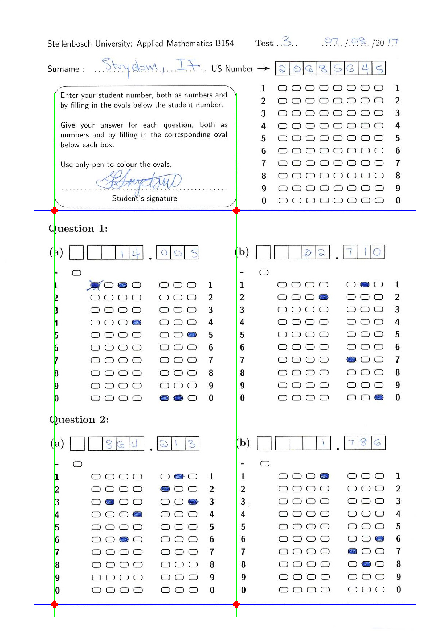
\includegraphics[width=14cm]{RadonResults}\\
  \caption{Four markers found from applying Radon transforms.}
  \label{fig:radonResults}
\end{figure}

\subsection{Initial filtering and orientation detection}
\label{sec:InitImageFilter}

To check if and image is upside down the software first needs to find relevant contours on the page. The contours are then filtered out if it does not loosely match the characteristics of a bubble or character block. This is done in 5 steps:

\begin{enumerate}
\item Threshold the image by making all the pixel values either white (lower that the mean) or black (higher that the mean)
\item Do contour analysis on the image to find all the contours, using the python library OpenCV.
\item Filter through the contour array to filter out all contours that are not approximately the size and aspect ratios desired.
\item Save these contours for later use.
\item Determine if more contours lie above the middle of the image. This is true if the image is the right way around. Rotate the image by 180$^{\circ}$ otherwise.
\end{enumerate}

It is important to note that there are still unwanted contours in the list, but for now this reduced list is sufficient. Once the list is found the software counts the number of contour centrepoints below and above the image center. Figure \ref{fig:reduced} shows the resulting contours found in the image. As can be seen in the figure more bubbles should be below the horizontal center line, for the image to be the right side up. The next step will now be to determine the coordinates of the answers the student wrote down. To do this the template is first located in the image. This process is described in Section \ref{sec:RadonTransform}.

\begin{figure}
  \centering
  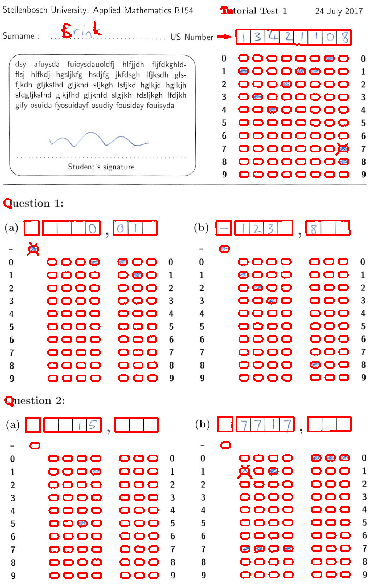
\includegraphics[width=14cm]{Reduced}\\
  \caption{Reduced contours in image.}
  \label{fig:reduced}
\end{figure}

\subsection{Radon Transform}
\label{sec:RadonTransform}
(Maak 'n symbols page)
The Radon transform is an integral transform that can be represented by a series of line integrals over a function $f(x,y)$. These transforms are commonly used in CT scans. Mathematically this transform is defined as $$G(r,\theta) = \int_{-\infty}^{\infty} \int_{-\infty}^{\infty} f(x, y) \delta(x\cos(\theta) + y\sin(\theta) - r) dx dy.$$Where $r$ represents the perpendicular offset of the line and $\theta$ the angle of the line. $x$ and $y$ represents a 2D space within which the function $f(x,y)$ is defined.  A visual interpretation of this transform can be seen in Figure \ref{fig:RadonT}.  

\begin{figure}
  \centering
  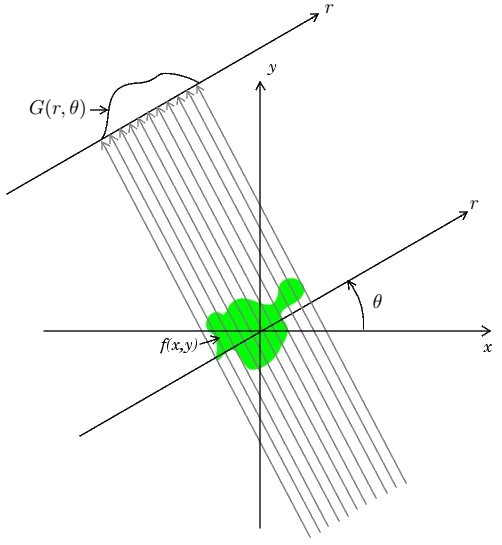
\includegraphics[width=14cm]{RadonT}\\
  \caption{Radon transform applied on a 2 dimensional area, from \citet{radon}}
  \label{fig:RadonT}
\end{figure}

\subsection{Finding the template}
\label{sec:findTemplate}

In this project a Radon transform is calculated at specific intervals of the gradient. Each gradient interval will thus generate a 1 dimensional array of values corresponding with the pixel intensities along the lines that are being summed, as seen in Figure \ref{fig:RadonT}. This method is used determine where the 2 horizontal and 2 vertical lines are located, as mentioned in Section \ref{sec:orientDetect}. 

To find the first two horizontal lines the Radon transform is applied at a angle of 90$^{\circ}$ and then incremented by a small amounts for the next transform. Black lines will cause a spike to appear on the Radon transform when it is summing parallel with that black line. Thus by finding the transform angle value that present this maximum value. The rotation of the template can be found. The two maximum values that is recorded at this angle is can then be interpreted as the locations of the two horizontal lines. After the correct angle is found the two vertical lines can be found by applying a Radon transform at a angle 90$^{\circ}$ clockwise from the previously calculated angle. Those two values then provides the relative locations of the two vertical lines. Now the four reference point shown in Figure \ref{fig:radonResults} can be calculated. Once the reference points are found the image is rescaled and orientated to the original template size and orientation for further processing. In Figure \ref{fig:rotate} the corrected image is shown, before it gets processed.

\begin{figure}
  \centering
  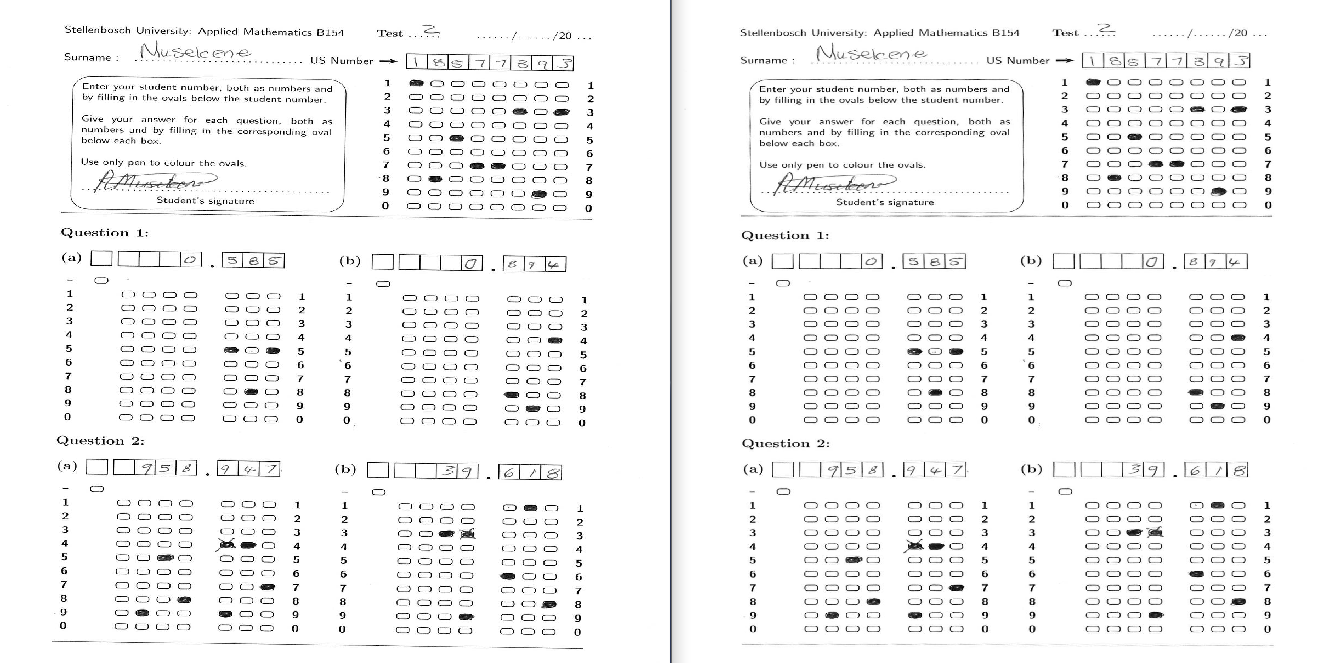
\includegraphics[width=14cm]{Rotation}\\
  \caption{Result in rotation after applying radon transform.}
  \label{fig:rotate}
\end{figure}

Once the template is found the bubble values and digit blocks can be determined, using reference location. These reference locations were calculated in preprocessing done on an empty template. Figure \ref{fig:FinalEstimate} illustrates the final estimation of all the bubbles in the template. The estimated bubble centres are coloured red, while the green points represent the centres of all the remaining contours.

\begin{figure}
  \centering
  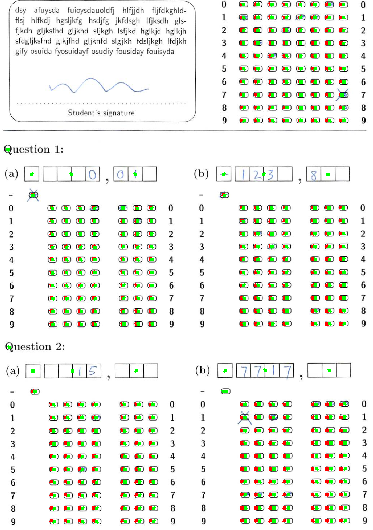
\includegraphics[width=14cm]{FinalEstimate}\\
  \caption{Detection of template in image and estimation of bubble locations.}
  \label{fig:FinalEstimate}
\end{figure}

Now that all a list of possible bubble contours are found, the next challenge is to find one contour for each bubble. This is discussed in the next section.

\section{Bubble detection and processing}

To find the location of each bubble in the image, the system simply takes the contour closest to the estimated bubble location. This can be done in an efficient manner by sorting the contours by their locations. Searching through the contours now becomes linear and of complexity O(n), where n is the number of bubbles. This means that the processing time to find these bubbles is linearly related to the number of bubbles in the template image. 

Next the data in each contour needs to be processed and stored. The first type of evidence is calculating the average pixel intensity inside the contours. If this value is high the bubble is most likely coloured in or crossed out. The advantage of using the closest contour as the bubble's estimated location, over conventional methods now becomes apparent. In conventional methods an estimated area is calculated where the bubble is most likely to be located. This becomes problematic if the system needs to know if the bubble has been crossed out, as only data about pixel intensities are present. 

Using contour analysis, information about the shape of the bubble entry is also provided. Thus by drawing the smallest possible block around the contour, that still covers every value inside the contour, an area can be calculated. This area becomes large when a answer is crossed out, due to the lines stretching outside the initial bubble. By inspecting the area value, the system can successfully determine if the bubble is filled in and crossed out.

\section{Data processing and grading}

The previous section now allows each bubble to be classified into 3 categories namely, empty, completely filled in and crossed out. An additional category of partially filled in will also be introduced, as it aids grading of tests where students write lightly. An algorithm to determine what bubble was chosen can now be described as follows:

\begin{enumerate}
\item Count the number of completely filled in answers in each column. Store the position of that entry for later use.
\item If there are no completely filled in answers, count the amount of partially filled in answers and override the previous values.
\item If the previous result is 0, set the output value for that column to 0.
\item If step 2 or 3 presents a value greater that 1, save the answer sheet to a clashlist to be evaluated manually once the automatic grading of the test are completed.
\end{enumerate}


\section{Conclusion}

This chapter provided an overview of a basic automatic test grading system using image processing and computer vision. The system can achieve acceptable results using only these techniques.

The following chapter will focus on applying additional machine learning techniques to further improve the accuracy of grading these test. Two new test templates will also be introduced. (maak seker jy het daaroor gepraat).